\documentclass[letterpaper,notitlepage,twoside]{article}

% Basic imports, increase margins...
\usepackage[margin=0.75in]{geometry}
% Finite State Machine stuff

% Format tables nicely
\usepackage[latin1]{inputenc}
\usepackage{array}

\usepackage{amsfonts}
\usepackage{amssymb}
\usepackage{amsmath,amsthm}
\usepackage{tikz}

\renewcommand{\implies}{\Rightarrow} % redefine command "implies"
\renewcommand{\iff}{\Leftrightarrow} % double arrow
\newcommand{\maps}{\rightarrow} % define command "map"
\newcommand{\union}{\cup}
\newcommand{\intersect}{\cap}
\newcommand{\N}{\mathbb{N}} % natural number
\newcommand{\Q}{\mathbb{Q}} % rational number
\newcommand{\R}{\mathbb{R}} % real number
\newcommand{\Z}{\mathbb{Z}} % integers
\newcommand\tab[1][1cm]{\hspace*{#1}} %\tab command

% Add more packages that you use here...

\begin{document}
\title{Homework 20}
\author{Brian Knotten, Brett Schreiber, Brian Falkenstein}
\maketitle
\section*{3}

\section*{5}
To prove that if an algorithm for one of Undirected Graph Isomorphism, Directed Graph Isomorphism, and Mixed Graph Isomorphism implies that they all do, the following reductions need to be made:
\begin{itemize}
    \item Undirected Graph Isomorphism $\leq_p$ Mixed Graph Isomorphism
    \item Mixed Graph Isomorphism $\leq_p$ Directed Graph Isomorphism
    \item Directed Graph Isomorphism $\leq_p$ Undirected Graph Isomorphism
\end{itemize}
Using these three reductions, if any of the problems has a poly-time algorithm, then they all do, since, given one poly time algorithm, each reduction implies the existence of a second poly-time algorithm for any of the problems, and the third poly-time algorithm can be derived from the second poly-time algorithm.
Here are the reductions:
\subsection*{Undirected Graph Isomorphism $\leq_p$ Mixed Graph Isomorphism}
Assume there exists an algorithm for Mixed Graph Isomorphism called $MISO$. Then it is possible to construct a poly-time algorithm for Undirected Graph Isomorphism $UISO$ as follows:
\\\\
$UISO(G, H):$\\
\tab return $MISO(G, H)$
\\\\
A purely undirected graph can be thought of as a special case of a mixed graph, so an algorithm for Mixed Graph Isomorphism works just as well on inputs that only have directed edges. Moreover, since $MISO$ is poly-time, and since $UISO$ makes no transformations from input to input or from output to output, then $UISO$ is also poly-time.

\subsection*{Mixed Graph Isomorphism $\leq_p$ Directed Graph Isomorphism}
Assume there exists an algorithm for Directed Graph Isomorphism called $DISO$. Then it is possible to construct a poly-time algorithm for Mixed Graph Isomorphism $MISO$ as follows:
\\\\
$MISO(G, H):$\\
\tab Let $G' = Directed(G)$\\
\tab Let $H' = Directed(H)$\\
\tab return $DISO(G', H')$
\\\\
Where $Directed$ is a supplementary function as follows:\\
$Directed(G):$\\
\tab for each undirected edge $e$ between $u$ and $v$ in $G$:\\
\tab\tab add a directed edge from $u$ to $v$ into $G'$ and\\
\tab\tab add a directed edge from $v$ to $u$ in $G'$\\
\tab return $G'$
\\\\
An mixed graph can be thought of as a special case of a directed graph where each undirected edge corresponds to two mutual directed edges. Since two directed graphs can only be isomorphic if they both share these pairs of mutual directed edges, the algorithm remains correct after the input has been transformed. Since this transformation is polynomial in the number of edges, and since the output does not need to be transformed, then $UISO$ is also a poly-time algorithm.

\subsection*{Directed Graph Isomorphism $\leq_p$ Undirected Graph Isomorphism}
This reduction is the most sophisticated and requires the use of a gadget for transforming a directed graph $G$ into an undirected graph $G'$.

For each vertex $v$ in $G$, $G'$ contains the following subgraph:\\
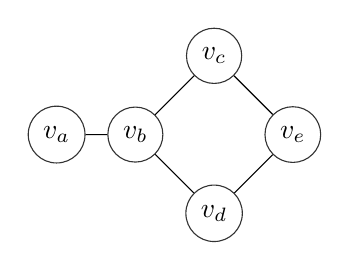
\begin{tikzpicture}
    \node[circle,draw=black!80] (a) at (0, 1) {$v_a$};
    \node[circle,draw=black!80] (b) at (1, 1) {$v_b$};
    \node[circle,draw=black!80] (c) at (2, 2) {$v_c$};
    \node[circle,draw=black!80] (d) at (2, 0) {$v_d$};
    \node[circle,draw=black!80] (e) at (3, 1) {$v_e$};
    \draw (a) -- (b) -- (c) -- (e);
    \draw (b) -- (d) -- (e);
\end{tikzpicture}
\\\\
Any directed edge from $u$ to $v$ in $G$ corresponds to an undirected edge between $u_a$ and $v_e$ in $G'$. This means that all edges outgoing $v$ in $G$ correspond to a "source" edge of $v_a$ in $G'$ and all edges going into $v$ in $G$ correspond to a "destination" edge of $v_e$. The subgraph gadget must be assymmetrical in order to distinguish these source and destination vertices.
\\\\
So if there exists a poly-time algorithm for Undirected Graph Isomorphism $UISO$, then there also exists a poly-time algorithm for Directed Graph Isomorphism $DISO$ as follows:
\\\\
$DISO(G, H):$\\
\tab Let $G' = $ undirected transformation of $G$ as described above\\
\tab Let $H' = $ undirected transformation of $H$ as described above\\
\tab return $UISO(G', H')$
\\\\
Since a directed edge corresponds to an edge from a source vertex to a destination vertex, then the transformed graphs are isomorphic iff the directed graphs are isomorphice. Moreover, the transformation requires a constant factor (5) vertices for a single vertex in the directed vertex, so the transformation of the inputs takes poly-time, and therefore $DISO$ is poly-time.
\end{document}
